\chapter{Simple questions, complex answers}
\label{chap:simple-questions-complex-answers}

In this chapter we are going to discuss some simple queries that are
very complex to express using existing SQL dialects for ESP
systems. We will try to understand the reasons for this difficulty and
propose solutions to eliminate it.

\section{Events are discrete, state is continuous}
\label{sec:acme-problem}

In the context of ESP applications, events are always discrete
entities, because they have a well defined position in time and the
information they carry becomes invalid outside that position. This
works for many scenarios that are discrete by nature --- earthquake
reports, orders placed in an online store, heart beats or even noise
readings sampled periodically, just to name a few. However, some
systems are truly continuous and the values reported by an event
influence what we know about the system and what we can conclude about
its state. Examples include price change reports, where we know that
the price of a product will remain the same until a later event
signals a change, temperature readings by a smart sensor that issues
reports only when the temperature differs by 0.1 degrees from the one
in the previous notification, or a goal scored in a football match
that updates its result until another goal is scored or the match
ends. Unfortunately, the semantics employed by ESP systems don't work
so well in these cases.

To see why, let's begin with a small example. Suppose we build an ESP
application to monitor noise-levels in a street, measured by a sensor
every 10 minutes. This application receives the following two events
and no others:

\begin{tabular}{ |l|r| }
  \hline
  Timestamp & Noise (dB) \\
  \hline
  11:00 am & 70 \\
  11:10 am & 50 \\
  \hline
\end{tabular}

Suppose further, that our application is interested in analyzing the
last 20 minutes of data and, to achieve that, uses a regular temporal
sliding window like the one discussed in section \ref{sec:sql}. Figure
\ref{fig:window-contents} shows the contents of this window between
11:00 am and 11:30 am.

\begin{figure}[htpb]
  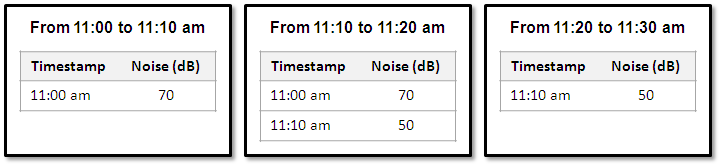
\includegraphics[width=\textwidth]{window-contents.png}
  \caption{Contents of the 20 minutes sliding window between 11:00 am
    and 11:30 am.}
  \label{fig:window-contents}
\end{figure}

By querying this window, we are now able to answer a few
questions. For example, at 11:10, the loudest reading registered
during the past 20 minutes was 70 dB, while 10 minutes later the
first event expires and the answer becomes 50 dB. Note that you cannot
ask for the loudest moment in the last 20 minutes, because a noisy
ambulance may have passed while the sensor was idle. That is, you
cannot assume anything in the time that goes from one event to
another. However, given the data that is available, the application
returns the correct answer.

This application is so successful that we are asked to adapt it to
monitor the stock market. Our clients are investors who want to be
able to make good decisions as quickly as possible and, to do so, our
application must handle events informing about every single
transaction. Suppose the application is deployed and receives the same
two events from the previous example, where instead of representing
noise-levels, they now refer to the value of ACME stock actions. Using
the same 20 minutes window, we may try to compute the highest price
attained by ACME during this period. At 11:10 am, the application will
return \$70, while at 11:20 am the answer will change to \$50, just
like in the previous example. However, this answer is known to be
wrong because the price remained at \$70 until 11:10 am and thus, the
answer should remain unchanged until 11:30 am\footnote{Strictly
  speaking, this is not how the stock market works: prices are not
  continuous and any investor may buy or sell for how much as he
  pleases. We ignore this detail because there are many situations --
  even in the stock market -- where it makes sense to treat discrete
  values as continuous.}. Despite using the same input data, posing
the same question and obtaining the same two results, one was correct
while the other was wrong.

\begin{figure}[h]
  \center
  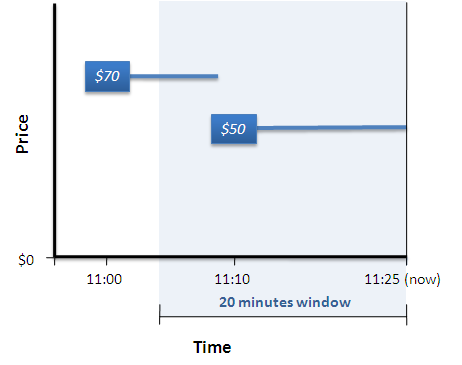
\includegraphics[width=0.7\textwidth]{outside-window.png}
  \caption{Evolution of ACME stock prices in the scenario described in
    the text. Values in boxes represent the two events received at
    11:00 am and 11:10 am. As you can see, at 11:25 am the first event
    lies outside the window and the engine will not consider it, even
    though its value remained valid throughout part of the window.}
  \label{fig:outside-window}
\end{figure}


The central difference between these two examples, pertains to what
can be assumed between events. There are three different cases:

\begin{itemize}
\item Between events the value is undefined. This is what happens when
  the value is discrete by nature --- the sender of a network packet
  is undefined when there is no network traffic ---, or when the event
  generator is sampling a continuous entity, like the noise sensor of
  the first example. We will refer to this as the \emph{pulse}
  semantics;
\item The value remains constant until the next event modifies
  it. This is valid if the value represents a new state, like the
  price of ACME stock actions, that remains the same between two
  updates. As such, we will call this the \emph{state-changes}
  semantics. Some continuous distributions that are known to be smooth
  may also be modeled under these semantics. For example, temperature
  may be assumed to remain constant between two updates, unless sudden
  variations not reported by the sensors are problematic;
\item In some rare cases, the value between events may be approximated
  by a well known mathematical function.
\end{itemize}

Existing languages adopted the pulse semantics by design. This is a
natural choice if we consider events as isolated occurrences. However,
if events represent changes in state, these languages will disappoint
because the developer has to manage this state manually. This can be
seen in Appendix \ref{sec:acme-problem-solution}, where a solution to
the ACME stocks problem, implemented in Coral8 CCL, is shown. The
algorithm creates two windows: the 20 minutes window and another
window that will contain the newest event older than 20 minutes (i.e.,
the event that most recently expired from the 20 minutes
window). Then, we perform a \verb=full outer join= between both
windows (\verb=union= would be more appropriate, but Coral8 doesn't
support it) and calculate the maximum price in either of them. As you
can see, this solution is quite verbose, which would be OK if only
there weren't so many situations like this, where the values are
continuous and must be handled with special care.

A slightly modified version of the ACME problem was posed on an online
community where researchers and vendors participate
\cite{simple-problem} \cite{simple-problem2}. It generated a lengthy
(more than 60 messages), interesting and sometimes funny
debate. Several vendors replied --- including Oracle, Aleri, Coral8
and Esper ---, and tried to find a good solution using their
products. In our opinion, they failed because their solutions were
verbose (like the Coral8 one above), inefficient or wrong. In the end,
some participants concluded this was not an event processing problem
anyway because it involves state and tried to dismiss it as
irrelevant, while others argued that queries like these show up every
day and if ESP engines can't solve them, their usefulness is reduced.

We agree that existing ESP engines shouldn't be applied to problems
like these, not because they don't matter, but because these engines
were not prepared to solve them --- even if they are able to do so
with more or less trouble. Instead, we believe these problems call for
a new language, encompassing both pulse and state-changes semantics,
that provides first-class constructs to deal with them.



\section{Defective products detection -- the ``too muggy'' query}
\label{sec:defective-products}

Another class of problems that are reasonable in the context of ESP,
but are difficult to solve by current systems, are those where the
developer needs to know for how long a certain condition was true (or
false). For example, imagine the following scenario, attributed to
Andrew Witkowski from Oracle and illustrated in figure
\ref{fig:factory}: a factory has several rooms, every room has at
least one humidity sensor and one temperature sensor. Furthermore,
products contain a RFID tag that is read by RFID sensors placed at the
entrance of each room. All these sensors send their readings to a DSMS
that needs to answer the following question: ``Which products stayed
more than 10 minutes (not necessarily consecutive) at more than 20
$^{\circ}$C and 80\% of humidity?''. These products are defective and
mustn't go to the shelves.

\begin{figure}[htbp]
  \center
  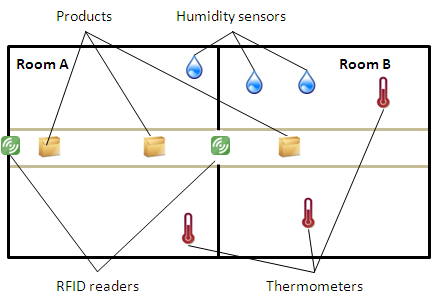
\includegraphics[width=0.6\textwidth]{factory.png}
  \caption{The factory outline.}
  \label{fig:factory}
\end{figure}


A solution for a simplification of this problem, written in Coral8
CCL, is shown in Appendix \ref{sec:defective-products-solution}. This
solution does not take humidity into consideration and assumes there
is only one sensor per room. The algorithm is simple: for each
product, we keep one counter with the time the product spent above 20
degrees, as well as the timestamp for when this counter was last
updated. When a product leaves a room, we update its counter if the
temperature in the previous room was higher than 20, and set the last
updated timestamp to the current time, given by the \verb=now()=
function. When the temperature changes, we do the same thing for all
products in that room.

This solution is quite long (3 pages of SQL-like code) as it is and it
still doesn't solve the original problem. Worse, the solution is long
and complicated because it needs much more than the standard operators
the language provides, which means that it is not possible to express
it using a few queries. Instead, the only way is resorting to an
algorithmic solution where the developer needs to explicitly write
down all the steps of the computation. This is, however, contrary to
the declarative nature of SQL and one has to wonder if using a
procedural language such as Python or Java -- where the developer is
able to create new operators better suited for the problem at hand --
wouldn't result in a simpler program. One may argue that this is a
difficult problem and the solution can't be simple
anyway. Nonetheless, it is a good exercise to analyze this piece of
code to see what else is wrong with it.

Let's begin by thinking about what would have to be modified to
support humidity. Naturally, we would have to create a new stream ---
\verb=hum_readings= --- that receives humidity readings from
sensors. Then, it would make sense to create a window to keep the last
humidity reading per room, analogous to the \verb=RoomTemperature=
window for temperatures. When the humidity changes, we need to
generate new events with the identifier of the room and its old
humidity, just like we do now when a product switches rooms or when
the temperature changes. When an event arrives in this stream, we
check if the previous humidity was greater than 80\% and if the
current temperature is above 20 degrees. If both conditions hold, we
may finally proceed to update the product's counter as well as its
last updated timestamp. Unfortunately, we are not done yet: it is also
necessary to modify the other queries, that are triggered when the
temperature changes or when the product switches rooms, to take the
current humidity level into consideration. Thus, adding new sensors
implies not only writing new queries, but also modifying existing
ones. Clearly, this approach does not scale\footnote{``scale'' here
  refers to the source code, not to the performance of the solution.}
as extensive rewrites are necessary every time the requirements are
modified. Software engineering best-practices dictate that, if
something like this happens, then the code is not modular enough or is
using the wrong abstractions.

The solution for this problem implemented in the appendix shows some
of these symptoms. There, besides the two input streams and the window
with the counter per product, we create two other windows and two
temporary streams. The windows contain the current and previous
temperatures of each room and the current and previous room for each
product. Thus, these windows are used to maintain the state of the
system. To support humidity, we would need a third window to maintain
the current and previous humidity level for each room. Note how
information (temperature and humidity) for a given entity (the room)
becomes scattered across several windows. To correlate temperature
with humidity, one would need to join these windows and then group by
the room's id. Thinking from an object-oriented point-of-view, it is
easy to see that this query would be greatly simplified if there was
some way to define \verb=Room= objects with properties such as
\verb=temperature= or \verb=humidity=, and use these objects in
queries, just like regular events. Moreover, one could instruct the
system to create the objects and manage their attributes
automatically, by looking at the right events. We could take this one
step further by supporting relationships between objects, akin to what
Object-Relational Mapping (O/RM) tools such as Hibernate
\cite{hibernate:www} do for regular databases. This way, each
\verb=Room= object would possess a list with its \verb=Product=s and
each \verb=Product= would include a reference to the \verb=Room= where
it is at. With these changes, finding the current temperature of the
room where a product is would be as simple as typing
\verb=product.room.temperature=.

% TODO: Make picture of the algorithm

As for the two temporary streams, their events are created when the
products switch rooms or when the temperature of a room changes, and
contain the previous room id or the previous temperature. These
streams are not strictly necessary as their code could be directly
inserted into the \verb=FROM= clause of the queries that use
them. However, this would not be a good idea as it would quickly
result in unreadable code. To avoid creating big and complex queries,
developers partition them into smaller ones connected by temporary
streams. Thus, streams end up being used as variables to store the
intermediate results of computations. But streams aren't a suitable
replacement for all kinds of variables. In procedural programming
languages, programmers can choose among primitive variables (int,
float, string, \dots), arrays, dictionaries, lists, sets and, why not,
objects. Certainly, streams and windows alone could be used to
simulate all these kinds of constructs, but they're just not the right
tool for \emph{every} job.

\section{Semantic windows}
\label{sec:semantic-windows}

Suppose that ACME stock is worth more than \$70 during some interval
and you want to know what was the average of its price during that
interval. Solving this problem using current technology is not so
difficult. Most ESP products include some kind of event detection
feature that allows the search for patterns of events. To obtain an
answer, we could find the event where ACME stocks passed the \$70
mark, then find all the events where the price stayed above that
threshold and, finally, find the event where they descended below
\$70. With all these events, we could then proceed to calculate the
average price.

There are two problems with this approach. The first is that the
detection of the boundaries of this interval may itself involve the
detection of another complex pattern. For example, to discover the
event where the price rose above \$70, one needs to compare some event
with the one that preceded it. The second problem is that these
complex event detection features work by first detecting the pattern
and then processing it. Thus, while the price remains above \$70, the
engine keeps all the events in memory and only when the price goes
below that mark will it proceed to calculating the average. This is
suboptimal, because the engine could keep a temporary sum of the
prices and a temporary count of the number of events received. These
two numbers are enough to generate the average and thus, the events
themselves could be discarded immediately.

A better way to solve this last problem is through \emph{semantic}
windows \cite{semantic-windows}. These are windows whose endpoints are
fixed by events, instead of being defined by time or number of
elements. Currently, no product supports this type of windows. Using
semantic windows we could instruct the engine to open the window when
the price ascends above \$70 and close it when it finally descends
below that mark. The advantage of this approach is that all windows
are closed eventually --- i.e., if the opening pattern is found, then
we are sure that there will be a corresponding closing event. Thus,
the engine knows a priori that there will be a successful match for
this window and may begin calculating the average right away, while
saving space by discarding the events that will be no longer needed.

Regarding the first problem --- detecting the moment the price passes
the threshold in either direction ---, notice that stock prices belong
to the state-changes class of problems discussed in section
\ref{sec:acme-problem}. Hence, the price evolution of ACME stocks may
be plotted using a continuous step-function over time, similar to the
one in figure \ref{fig:outside-window}. Our problem then becomes a
simple matter of cutting the plot horizontally where price equals 70,
ignoring the values below that value, and calculating the average for
the remaining plot. All of this could be done by the engine behind the
scenes, but only if it is smart enough to distinguish between pulse and
state-changes semantics.

\section{Summary}

In this chapter we have shown that there are problems where existing
languages perform poorly. We believe this happens because these
languages work at a very low level which forbids the developer to
think in terms of higher abstractions. In summary, the issues found
were:

\begin{itemize}
\item The pulse semantics, adopted by all engines, are unsuitable for
  many problems where the events represent state-changes of some kind;
\item It is difficult to decouple the various parts of a solution in
  such a way that introducing a new feature does not require rewriting
  part of the existing code;
\item Related data may be scattered across several streams and
  windows, forcing the developer to perform SQL operations --- in
  particular \verb=JOIN=s and \verb=GROUP BY=s ---, to join it
  together. We believe most of these queries could be made simpler by
  structuring the data in a different way, using objects;
\item In these languages, streams and windows are the only data
  structures available, while many algorithms would benefit from a wider
  choice;
\item Some problems require new operators -- semantic windows,
  operators to deal with time, new aggregators, etc -- but there is no
  way to create them.
\end{itemize}

It's not our purpose to claim that SQL, in general, is not well-suited
for ESP applications. However, we believe that ESP problems have their
own needs that require the availability of new data types, new
operators and different semantics, to the point where the resulting
language can hardly be called a SQL dialect anymore. Still, SQL has
benefits. For simple things, its declarative nature makes it very
expressive. Also, SQL querying capabilities are very powerful and
excel in many data processing tasks. It is understandable then, that a
new language should take some inspiration from SQL and borrow some
features to provide equally powerful constructs.
